%%%%%%%%%%%%%%%%%%%% author.tex %%%%%%%%%%%%%%%%%%%%%%%%%%%%%%%%%%%
%
% sample root file for your "contribution" to a contributed volume
%
% Use this file as a template for your own input.
%
%%%%%%%%%%%%%%%% Springer %%%%%%%%%%%%%%%%%%%%%%%%%%%%%%%%%%


% RECOMMENDED %%%%%%%%%%%%%%%%%%%%%%%%%%%%%%%%%%%%%%%%%%%%%%%%%%%
\documentclass[graybox]{svmult}

% choose options for [] as required from the list
% in the Reference Guide

\usepackage{mathptmx}       % selects Times Roman as basic font
\usepackage{helvet}         % selects Helvetica as sans-serif font
\usepackage{courier}        % selects Courier as typewriter font
\usepackage{type1cm}        % activate if the above 3 fonts are
                            % not available on your system
%
\usepackage{makeidx}         % allows index generation
\usepackage{graphicx}        % standard LaTeX graphics tool
                             % when including figure files
\usepackage{multicol}        % used for the two-column index
\usepackage[bottom]{footmisc}% places footnotes at page bottom

%
\usepackage{url}
\usepackage{amssymb}

% see the list of further useful packages
% in the Reference Guide

\makeindex             % used for the subject index
                       % please use the style svind.ist with
                       % your makeindex program

%%%%%%%%%%%%%%%%%%%%%%%%%%%%%%%%%%%%%%%%%%%%%%%%%%%%%%%%%%%%%%%%%%%%%%%%%%%%%%%%%%%%%%%%%

\begin{document}

\title*{Evaluating the Performance of Bitcoin Scaling Test Network}
% Use \titlerunning{Short Title} for an abbreviated version of
% your contribution title if the original one is too long
\author{Akihiro Fujihara and Takaaki Yanagihara}
% Use \authorrunning{Short Title} for an abbreviated version of
% your contribution title if the original one is too long
\institute{Akihiro Fujihara \at Chiba Institute of Technology, 2-17-1 Tsudanuma, Narashino, Chiba 275-0016, JAPAN, \email{akihiro.fujihara@p.chibakoudai.jp}
\and Takaaki Yanagihara \at Chiba Institute of Technology, 2-17-1 Tsudanuma, Narashino, Chiba 275-0016, JAPAN, \email{s1522313qq@s.chibakoudai.jp}}
%
% Use the package "url.sty" to avoid
% problems with special characters
% used in your e-mail or web address
%
\maketitle

\abstract{
Bitcoin Scaling Test Network (STN)は,ビットコインのスケーラビリティ問題を
On-chain技術で解決する為の実験ネットワークである.P2Pネットワーク上には
常に大量の取引が送信されており,巨大ブロックを生成する実験が行われている.
本研究ではSTNノードを構築することで,取引処理の稼働率やブロックチェーン
の分岐確率の推定を行った.その結果,推定稼働率は約1.04,推定分岐確率8.5\%
となった.
更にOP\_RETURNスクリプトを含む取引を1分に1回の高頻度で1週間の期間転送する
ことで取引処理性能を実験的に評価した.その結果,取引がBCに取り込まれる確率
は98\%となった.また取引が取り込まれるまでにかかる時間分布は長期的には
冪分布に従う傾向を確認した.
以上より,STNにおいても優先権付き待ち行列理論による考察が有効であると
考えられる.
(Tantative) 
 Bitcoin Scaling Test Network (STN) is an experimental network to solve the 
scalability problem of Bitcoin by using on-chain technology. 
 A large number of transactions are constantly sent over the P2P network, 
and miners generate huge blocks.
In this study, we estimated the occupancy rate of transaction processing 
and the fork probability of the blockchain by constructing STN nodes. 
 As a result, the estimated occupancy rate was about 1.04 and the estimated 
fork probability was 8.5\%.
 In addition, we experimentally evaluated the transaction processing 
performance by transferring many transactions containing the OP\_RETURN 
script once per minute for one week. As a result, the transaction processing 
probability was 98\%, and the latency distribution for transaction processing 
tends to follow a power distribution in the long period.
These results suggest that the priority queueing theory is also effective 
for STN.
}


\section{Introduction}
\label{sec:intro}


ビットコイン\cite{nakamoto}は2008年にP2P電子貨幣システムとして
提案され,翌2009年1月3日に創始ブロックが生成されて以来,利用さ
れ続けている.
Bitcoinの本質的に新しい利用価値は,取引にかかる手数料を極度に
安くする事によって実現できる(1円や1セント以下の)超少額決済 
(Micropayment) にある.このことによってインターネット上の様々
なサービスの利用時に,ほぼ0に近い(人々が支払いを行ったことを
気にしないレベルの)課金を沢山のユーザから集めることによって
サービス運営の為のコストを回収することが可能となる.
つまり超少額決済は,これまでにない新しい分散型経済の仕組みを
作ることができる潜在能力を持っている.

一方,ビットコインやブロックチェーン(BC)を用いたビジネスは
新しい分散経済の仕組みを構築する方向には全く進化していない.
Bitcoin Core (BTC) \cite{btc} は電子貨幣システムではなく,
投機目的の価値の貯蔵システムと化してしまった.
その背景には,現状のビットコインでは多数の超少額決済の実行が
事実上困難であるという理由がある.

BTCのブロックサイズの上限は1MBに決まっている.これより大きな
サイズのブロックは不当なものとみなされ,マイナーに拒否される
ことになっている.またビットコインの平均ブロック生成時間は
10分になるように難易度調整アルゴリズムによって制御されている.
従って,平均10分に1MB以下のブロックに取り込めるだけの取引しか
処理することができない.これは1秒あたり5〜7取引しか処理できな
い計算になることが知られている.
単純に平均ブロック生成時間を10分より短くしたり,ブロックサイズ
の上限を1MBより大きくすれば,この問題が解決するように思われる.
しかし,ブロックサイズを大きくすると,ブロックをP2Pネットワーク
上の全ノードに転送して共有する過程により時間がかかってしまう.
従って,平均ブロック生成時間を10分より長くしないとブロックが
P2Pネットワーク全体に行き渡る前に別のブロックが生成される確率が
あがる.従って,単純にブロックサイズを大きくしてもBCの分岐を
引き起こすことになる.分岐が起こるとProof of Work (PoW)を行って
ブロックを生成するノードのハッシュレート(単位時間あたりに
ハッシュ関数の計算を実行できる回数)が二種類のブロックのものに
分断されてしまい,将来的に排除されてしまうブロックの生成に大量
のハッシュパワーをかけてしまうことにつながり,ネットワーク全体
のブロック生成効率も下がる.
逆に平均ブロック生成時間を10分よりも短くしても,そのうちBCの
分岐が起こりやすくなり,同様の困難が生じる.
これらの理由により,単位時間あたりの取引処理性能を向上すること
には技術的な困難がある.この技術的な課題のことをスケーラビリティ
問題と呼ぶ.

ビットコインのスケーラビリティ問題を解決する方法も様々なものが
提案されている\cite{ZHZB2020}.
その中でもLightning network\cite{PD2016}のように,BC外で多量の
取引をまとめて実行し,その最終結果のみをBCに書き込むことで,
ブロックに取り込む取引量を減らすことによってスケーラビリティ
問題を回避する手法に注目が集まっている.このような解決手法は
BC以外の部分を工夫して困難を回避することから,Off-chainのスケー
リング技術と呼ばれる.
Off-chain技術は一見良いように見えるが,個々の取引処理がBCに
残らない.従って,Off-chainで処理した取引の改ざんが可能になって
くる.また,BCを導入することで取引の監査はブロック内の取引のみ
を確認すれば良い為,自動化が可能になるメリットがあったが,
Off-chain技術を適用すると,BC外の取引のチェックが既存と同じく
手動になってしまう為,BCのメリットを活かすことができなくなる.
つまりOff-chain技術はビットコインの元来の発想である,全取引を
公開することで監査可能性を最大限に発揮する考え方に逆行している.

一方,ビットコインはダークネット・マーケットにおける違法な取引
を行う手段として利用されてきた歴史がある.しかし,近年これらの
マーケットの支配人や利用者が逮捕される事例が数多く報告されてい
る\cite{silkroad,alphabay,welcome2video}.
これらの逮捕はビットコインが全取引を改ざん耐性を持たせて公開し
ている為に,法的な証拠として利用可能であることに起因する.
この観点から考えると,Off-chain技術が普及するほど,政府等が追跡
して監査することが不可能な取引が増えてしまい,ダークネット・
マーケットのような違法な取引の取り締まりが難しくなったり,マネー
ロンダリングの温床となりうる.法と倫理とのバランスを考えた時,
究極的にはBC上で全取引を処理するOn-chain技術によってスケーラビリ
ティ問題を解決することが求められる.

またIoTやAIとBCを組み合わせることで多様なデータやプログラムを
透明性の高いOn-chainで統合管理する応用も期待されている
\cite{SMNA2019}.
IPFSなどの分散ストレージ技術を使うことも可能ではあるが,
On-chain技術の発展によって取引処理性能が向上するほど,データや
プログラムの扱い方の自由度が広がる側面もある.

On-chainでスケーラビリティ問題を解決する為には,BCが分岐しない
ようにうまく制御しながら平均ブロック生成時間を短くするか,
ブロックサイズを大きくする必要がある.
bloXroute\cite{bloX}は,Blockchain Distribution Network (BDN)
という名称の,より大きなブロックをより短時間で伝搬させることが
可能なネットワーク層(Layer 0)をP2Pネットワークに接続することで,
スケーラビリティ問題を改善しようとする提案を行っている.

ブロックサイズを拡大する取り組みはBitcoin SV (BSV) \cite{bsv} の
スケーリングテストネットワーク (Scaling Test Network, STN) で
実験的な試みが行われている\cite{bitcoinscaling}.
巨大ブロックを生成するために大量の取引を送信する負荷テストも
行っている.
上述の通り,BTCのブロックサイズの上限は1MBであるのに対し,BSV
ではブロックサイズの上限を撤廃した.そのことにより,24時間あたり
の平均取引処理数が1,059 Transactions Per Second (TPS),
これまでに採掘された中で最も大きなブロックサイズは2.9GBと報告
されている(2021年2月9日閲覧確認).

本研究ではSTNのノードを構築することで,ブロックサイズの上限を
撤廃した環境における取引処理に関するデータ分析や性能評価実験を
行った結果について報告する.
本研究の貢献を以下に示す.
%
\begin{itemize}
  \item 待ち行列理論を用いることで取引処理の稼働率の時間変化を調べた.
	その結果,推定稼働率は殆どの時間帯で1を超えていることが分かった.
  \item bitcoin-cliの機能を用いることで,BCの分岐確率の推定を行った.
	その結果,BTCでは分岐確率が約2\%であることが計算されているが,
	BSV STNでは約8.5\%に増加していることが分かった.このことから,
	P2Pネットワークのノード全体にブロックを転送する時間は約53秒
	となることも計算により推定できた.
  \item OP\_RETURNスクリプトを含む取引を1分に1回の高頻度で転送した時に
	BCに取り込まれるまでにかかる時間を実測した.その結果,取引が
        BCに取り込まれる確率は98\%であり,その時間分布は冪分布に従う
	ような傾向が確認できた.また優先権付き待ち行列の理論と
	矛盾しない3/2の冪指数に従う傾向も確認できた.
\end{itemize}
%











\section{Related Works}
\label{sec:rworks}

\subsection{BCの分岐確率の計算}
\label{sec:fork}

ビットコインのブロック生成時間は指数分布に従うことが知られている.
%
\begin{equation}
	F(t) = P(T \le t) = \int_{0}^{t} \lambda e^{-\lambda t'} dt' = 1 - e^{-\lambda t}. \label{eq:exp}
\end{equation}
%
ここでパラメータ$\lambda$は平均ブロック生成時間の逆数である.
ビットコインの場合,平均ブロック生成時間は$1/\lambda=10$分$=600$秒
と決まっている.

またBTCのP2Pネットワークの90\%のノードにブロックが拡散されるまでに
かかる時間は$t = \tau_{fork} \fallingdotseq 12$ 秒であることが実測
値として知られている\cite{bloX}.
あるブロックがネットワーク全体に拡散される前に,別のブロックが生成
された時にBCが分岐してしまう.従って,ビットコインのBCが分岐する
確率は以下のように計算できる.
%
\begin{eqnarray}
  F(\tau_{fork}) &=& P(T \le \tau_{fork}) = 1 - e^{-\lambda \tau_{fork}} = 1 - e^{-12/600} \nonumber \\ 
		 &\fallingdotseq& 0.02. 
\end{eqnarray}
%
以上より,BTCのBCの分岐確率は約2\%であることが分かる.



\subsection{優先権付き待ち行列の理論}
\label{sec:priorityqueue}

優先権の高い客に対して先にサービスを行う優先権付き待ち行列において
稼働率$0 < \rho \le 1$の時,
優先権の低い客の待ち時間が冪指数$3/2$の冪分布に従い,その裾野が
指数分布のカットオフを持つことが理論解析の結果から知られている
\cite{OB2005}.
%
\begin{eqnarray}
  P(\tau) &=& \frac{A}{\tau^{3/2}} \exp(-\tau/\tau_0), \\
  \tau_0  &=& \frac{1}{\mu (1-\sqrt{\rho})^2}, \\
  \rho    &=& \lambda / \mu.
\end{eqnarray}
%
ただし,$A$は確率分布の規格化定数,$\lambda$は客の平均到着率,
$\mu$は平均サービス率である.

また稼働率が超臨界状態$\rho > 1$をとる時も同じ冪分布に従うことが
報告されている.$0 < \rho \le 1$の場合と異なる点は,$1-1/\rho$の
割合で待ち時間が無限の(サービスを永遠に受けることができない)
客が現れることである.

ビットコインにおける取引がBCに取り込まれるまでにかかる時間は
取引手数料に依存した優先権付き待ち行列理論で説明できることが
先行研究によって分かっている\cite{KK2019}.
このことから,BSV STNにおいても取引がBCに取り込まれるまでに
かかる時間分布も同様の性質を持つことが期待される.







\section{Bitcoin Scaling Test Network}
\label{sec:stn}


ビットコインのスケーラビリティ問題をOn-chain技術で解決する為の
実験場として,BSVではRegTest, Testnet以外の第3のテストネットと
してSTNが用意されている.
Testnetでは取引数が少ない為,ブロックサイズは小さい傾向にある
が,STNでは巨大ブロックを作るために大量の取引が定期的に送信さ
れている.
STNの未確認(=BCに取り込まれていない)取引件数の時間変化を
図\ref{fig:unconfirmed_tx}に示す.
%
\begin{figure}[tb]
  \vspace{-20mm}
  \begin{center}
    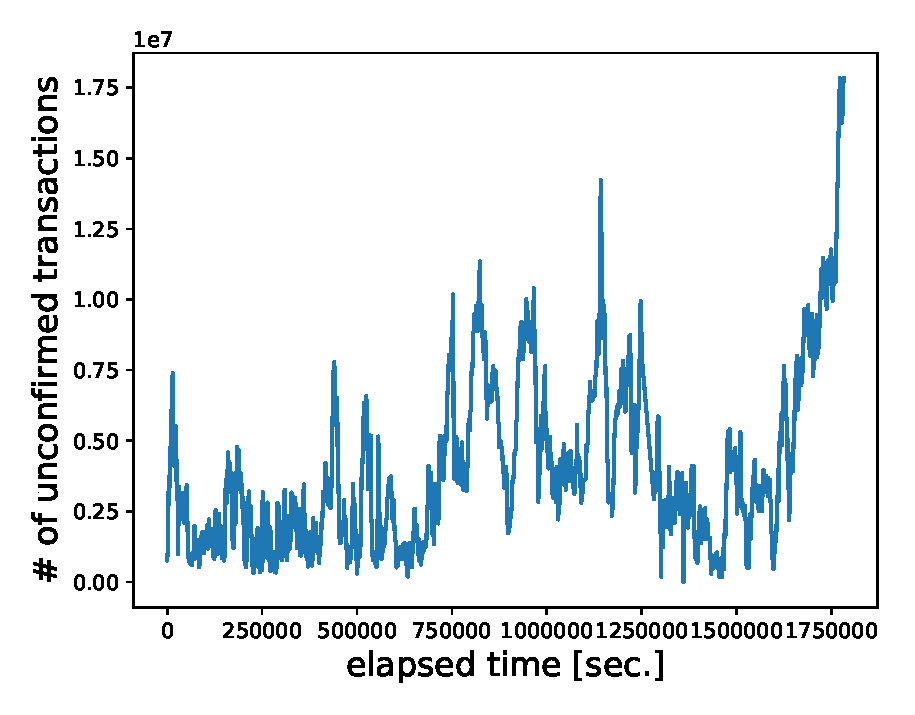
\includegraphics[width=85mm]{time_vs_tx-plot.eps}
  \end{center}
  \vspace{20mm}
  \caption{STNの未確認取引件数の時間変化}
  \label{fig:unconfirmed_tx}
  %  \ecaption{english caption is here}
\end{figure}
%
% TODO: check the format later
% ||
% \/
%\begin{figure}[t]
%\sidecaption[t]
%% Use the relevant command for your figure-insertion program
%% to insert the figure file.
%% For example, with the option graphics use
%\includegraphics[scale=.65]{figure}
%%
%% If no graphics program available, insert a blank space i.e. use
%%\picplace{5cm}{2cm} % Give the correct figure height and width in cm
%%
%%\caption{Please write your figure caption here}
%\caption{If the width of the figure is less than 7.8 cm use the \texttt{sidecapion} command to flush the caption on the left side of the page. If the figure is positioned at the top of the page, align the sidecaption with the top of the figure -- to achieve this you simply need to use the optional argument \texttt{[t]} with the \texttt{sidecaption} command}
%\label{fig:2}       % Give a unique label
%\end{figure}






ちなみにこの図を作成する元となったデータはwhatsonchain \cite{woc} 
で報告されているものを収集して利用している.
図\ref{fig:unconfirmed_tx}より,定常的に1,000,000以上の取引が
Transaction poolに存在していることが分かる.
また時々,取引数が10,000,000以上に達することも分かる.
BSVではOP\_RETURNスクリプトの利用をサポートしているが,
取引内容の大半は単純にアドレス間の送金になっている.

STNのネットワークは一般に公開されており,誰でもノードを構築して
P2Pネットワークに参加することができる.
ただしノード構築の為のシステム要求として,CPUは8〜16コア,
メモリは64GB(+64GB Swap),ハードディスクは3TB以上,インターネット
接続は上り下りとも1Gbit以上の性能が要求されている.
BCの総容量は2021年2月9日時点で2.4TBとなっている.
BSVのTestnetでは22GB,Mainnetでも284GB程度である為,比較すると
BCの容量が非常に大きいことが分かる.
またSTNのBCのブロック高は2021年2月9日時点で15,216となっており,
小さい.これは過去にBCの再編成(=ブロック高を下げて再開)を何度か
実施している為である.BSVのgithubの情報では2020年4月と11月に
BCの再編成が行われたことが記録されている.

またシステム要求からも分かるが,STNはCPUによるブロック採掘が可能
になっている.ブロック採掘の難易度の時間変化を
図\ref{fig:difficulty}に示す.
%
\begin{figure}[tb]
  \vspace{-20mm}
  \begin{center}
    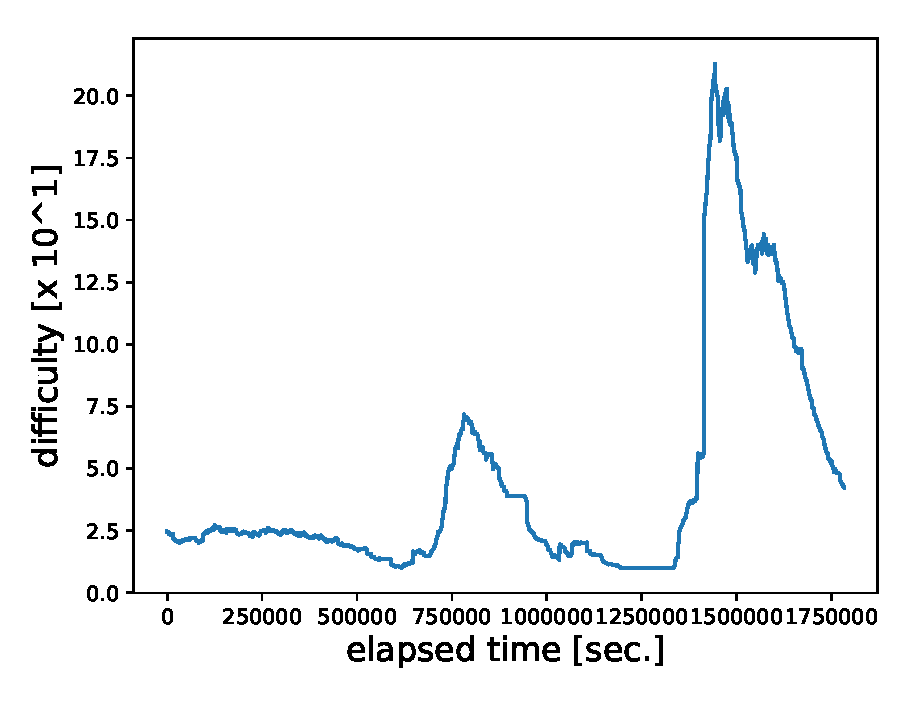
\includegraphics[width=85mm]{time_vs_difficulty-plot.eps}
  \end{center}
  \vspace{20mm}
  \caption{ブロック採掘の難易度の時間変化}
  \label{fig:difficulty}
  %  \ecaption{english caption is here}
\end{figure}
%
難易度は1〜数十の範囲で変化しており,容易に採掘が可能となっている.

STNでは最大ブロックサイズが10GBになるように設定することが推奨され
ている.またBitcoin scriptが使用可能なメモリの上限も2GBに設定する
ことが推奨されている.これまでに採掘されたブロックのサイズ分布を
調べた結果を図\ref{fig:block_size}に示す.
%
\begin{figure}[tb]
  \vspace{-20mm}
  \begin{center}
    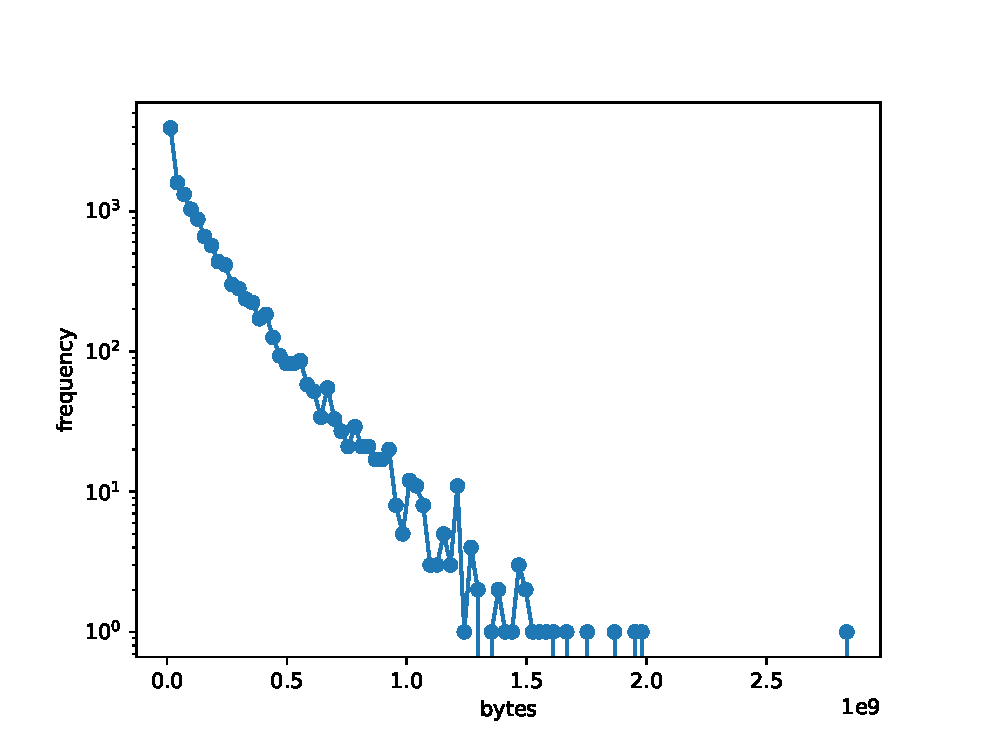
\includegraphics[width=85mm]{bsv_stn-block_bytes-semilogy2.eps}
    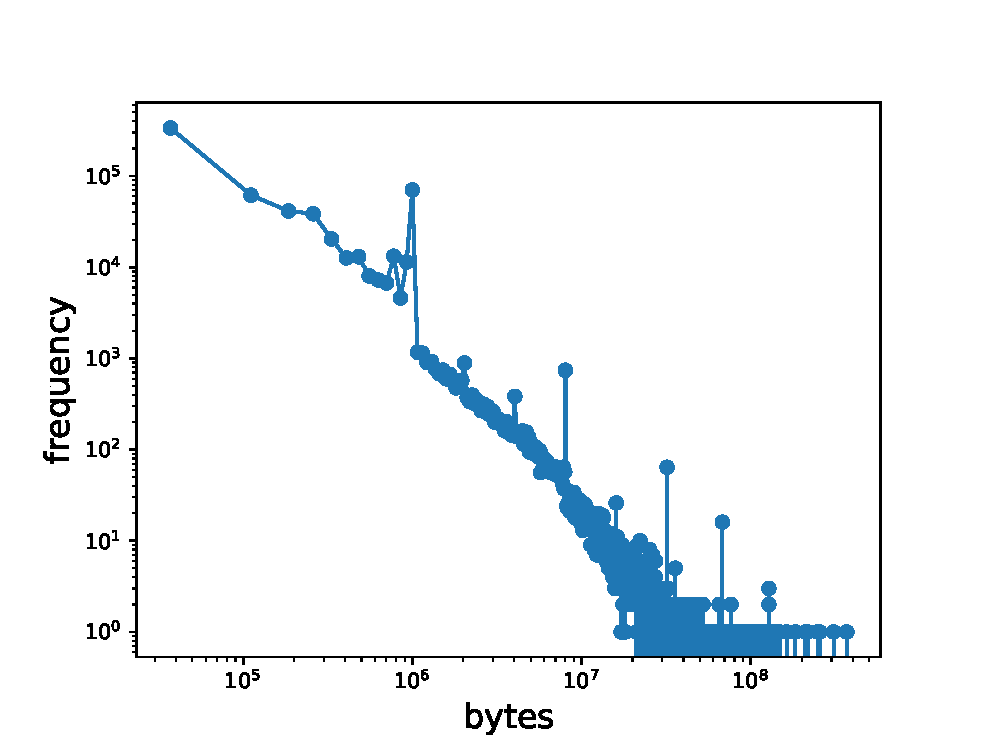
\includegraphics[width=85mm]{bsv_mainnet-block_bytes-loglog.eps}
  \end{center}
  \vspace{20mm}
  \caption{Bitcoin SVにおけるブロックサイズ分布(上図はSTN,下図はMainnet)}
  \label{fig:block_size}
  %  \ecaption{english caption is here}
\end{figure}
%
STNのブロックサイズ分布は指数分布に従っているように見える.
またこれまでに採掘された最大ブロックサイズは2.9GBになっている.
一方,図\ref{fig:block_size}の下図はMainnetでのブロックサイズ分布
になるが,興味深いことに指数分布よりも冪分布に従っているように見える.
また冪指数の傾向からPareto-Zipf則(=冪指数2の冪分布)に従っているよう
にも見える.
STNのコインには市場価値はないが,Mainnetでは市場価値を持つ.
分布にこのような差が生まれる理由については,よく分かっていないが,
市場価値を持つコインが入手できる場合,何らかの経済原理が働くことが
影響していると考えられる.

BSVは採掘者の評判を評価する観点から採掘したブロックに採掘者IDを記録
することを推奨している.この採掘者IDを参考にしてブロック採掘頻度の
ランキングを計算した結果を図\ref{fig:minerrank}に示す.
%
\begin{figure}[tb]
  \vspace{-20mm}
  \begin{center}
    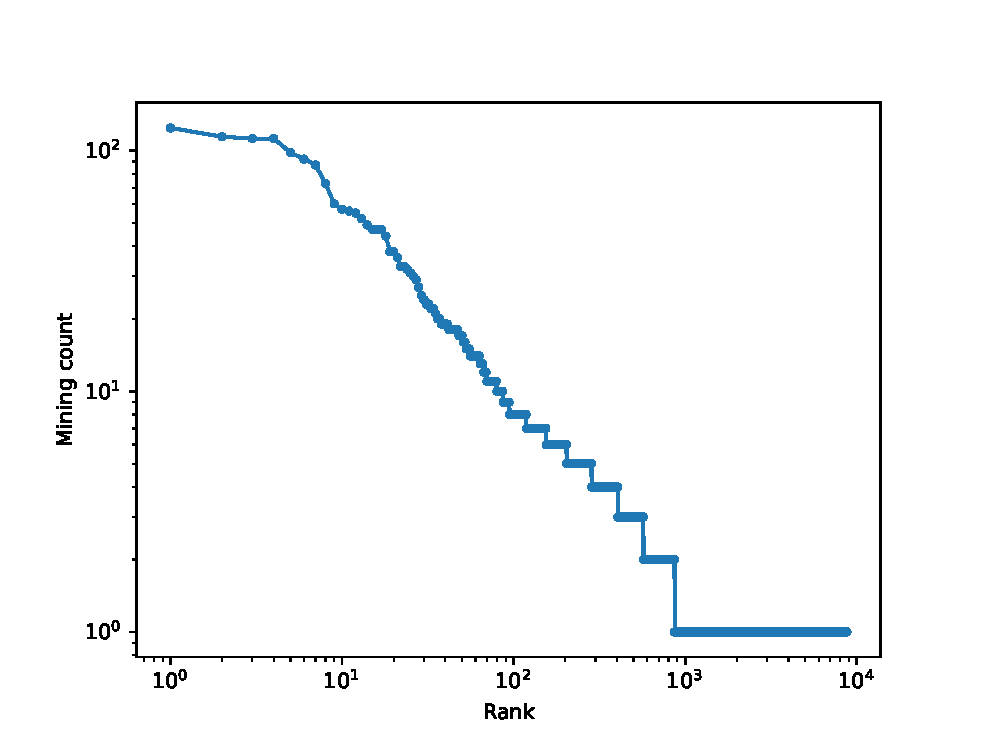
\includegraphics[width=85mm]{bsv_stn-block_miners-ranking-loglog.eps}
    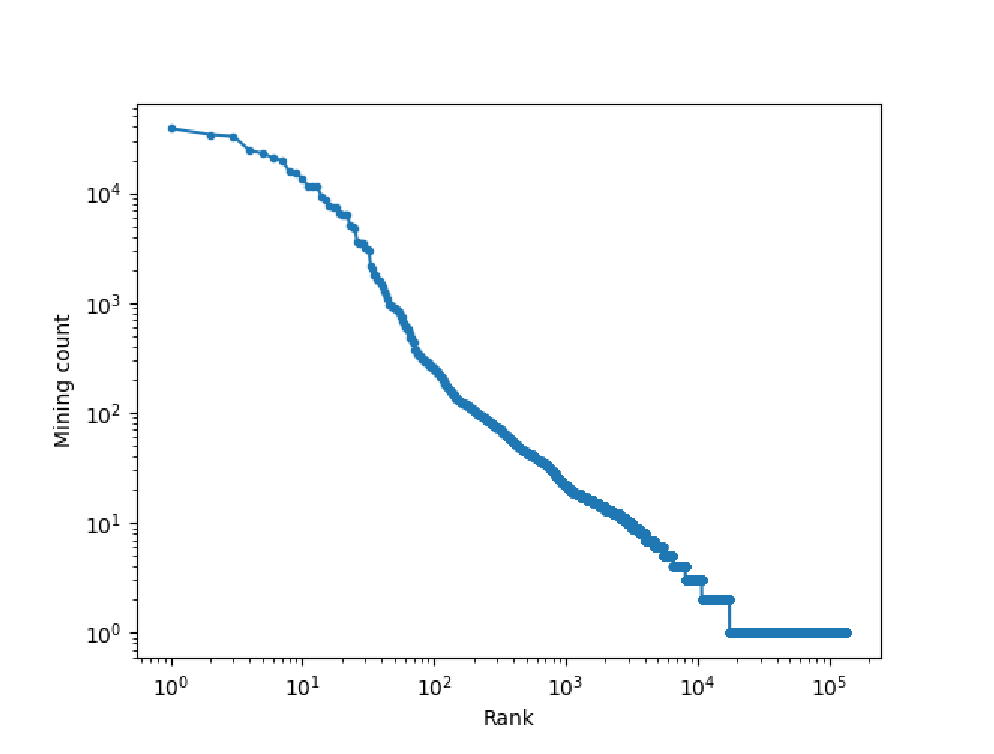
\includegraphics[width=85mm]{bsv_mainnet-block_miners-ranking-loglog.eps}
  \end{center}
  \vspace{20mm}
  \caption{採掘者IDを参考にして計算したブロック採掘頻度ランキング(上図はSTN,下図はMainnet)}
  \label{fig:minerrank}
  %  \ecaption{english caption is here}
\end{figure}
%
こちらはSTNとMainnetの両方とも冪分布に従っていることが確認できる.







\section{Performance Evaluation Experiments}
\label{sec:experiments}


\url{https://github.com/cit-fujihalab/stn_experiments}



\subsection{Experiment 1: }


図\ref{fig:unconfirmed_tx}における未確認取引件数の時間変化から,
STNの稼働率を推定した.
待ち行列理論に基づいて,STNの推定稼働率$\tilde{\rho}$の時間変化
を計算した結果を図\ref{fig:occupancyrate}に示す.
%
\begin{figure}[tb]
  \vspace{-20mm}
  \begin{center}
    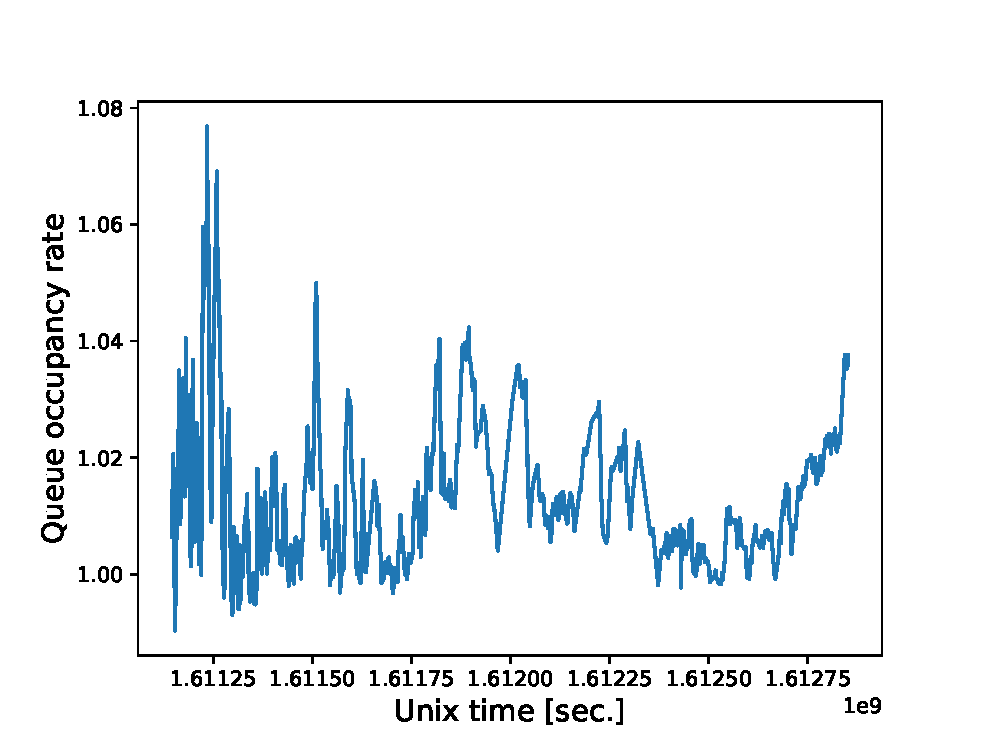
\includegraphics[width=85mm]{bsv_stn-rho-queue_occupancy_rate.eps}
  \end{center}
  \vspace{20mm}
  \caption{STNの推定稼働率$\tilde{\rho}$の時間変化}
  \label{fig:occupancyrate}
  %  \ecaption{english caption is here}
\end{figure}
%
推定稼働率は殆どの時間帯で1を超えていることが分かる.
この結果はBCに取り込まれない取引が存在することを示唆している.
また2020年11月4日〜2021年2月9日までのデータを用いて推定稼働率の
時間平均を取ると$\tilde{\rho} \fallingdotseq 1.04$となった.
この結果より,$1-1/\tilde{\rho} \fallingdotseq 0.0387$の確率で
BCに取り込まれない取引が出現していると考えられる.




\subsection{Experiment 2: }


STNのノードを構築してP2Pネットワークに接続すると分かるが,大きなブロック
が生成されたと思われるタイミングでBCの大きな分岐が起きてSafe modeとなり,
bitcoin-cliコマンドを使って送金ができなくなることがある.また一度大きな
分岐が起こると解消までに半日近くかかる場合もある.
そこでbitcoin-cli getinfoのerrorsの値を取得することで分岐が起きている時間
から分岐確率を推定する実験を行った.

2020年11月4日〜2021年1月13日の期間において,10秒に1回の頻度でerrorsの値を
収集した(合計594,880回).またBCが分岐している警告が出た回数を数えた.
その結果,以下の2種類の警告が出た.
%
\begin{itemize}
  \item Warning: The network does not appear to fully agree! We received
        headers of a large fork. Still waiting for block data for more details.
	(出現頻度は32,724回, 全体に占める割合は約5.5\%)

  \item Warning: The network does not appear to fully agree! Some miners
        appear to be experiencing issues. A large valid fork has been detected. 
	(出現頻度は17,782回,全体に占める割合は約3\%)
\end{itemize}
%
以上の結果より,分岐確率は約$(5.5+3=)8.5$\%と推定することができる.
これはBTCの約2\%の4倍超であることが分かる.
ちなみに同じ手法でBSV Mainnetの分岐確率を評価すると0\%となった.
また,式(\ref{eq:exp})において$F(t)=0.085$と$\lambda=1/600$を代入した時,
$t=\tau_{fork} \fallingdotseq 53$秒となることから,STNにおける平均ブロック
転送時間は約53秒になっていると推定することができる.




\subsection{Experiment 3: }


常に沢山の取引がTransaction poolにある状況で,取引がBCに取り込まれる
までにどの程度の時間がかかるかを実験により性能評価した.
実験期間を2021年1月7〜14日の1週間に設定し,期間中に分岐による取引送信
ができない場合を除いて常に1分に1回の頻度で,前の1分間にFlightradar24 
\cite{flightradar24} のADS-Bデータの収集ノードから千葉工業大学のある
津田沼周辺を飛行する民間航空機の位置情報を収集し,OP\_RETURNスクリプト
としてデータを含めた取引の送信を行った.
1取引あたりのサイズは63KB未満になるようにした.
また取引手数料は0.001BSVに固定した.
ちなみにBSVの取引手数料は1 satoshi/byte以上となっている.
昼間は民間航空機が多く飛行する為,取引データのサイズが大きくなるが,
夜間は殆ど飛行がない為,書き込むデータが無かった場合は取引の送信は
行わなかった.
実験結果に関するその他の詳細情報はGithub 
(\url{https://github.com/cit-fujihalab/stn_experiments})
に掲載した.

実験期間の経過時間と取引が取り込まれたブロック番号の対応関係を
図\ref{fig:exp3-1}に示す.
%
\begin{figure}[tb]
  \vspace{-20mm}
  \begin{center}
    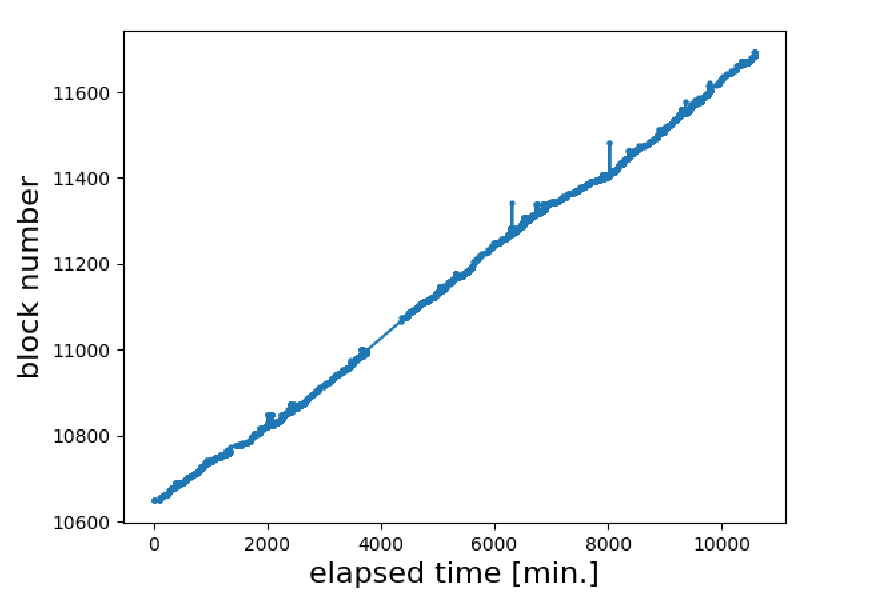
\includegraphics[width=85mm]{exp3-1.eps}
  \end{center}
  \vspace{20mm}
  \caption{経過時間と取引が取り込まれたブロック番号の対応関係}
  \label{fig:exp3-1}
  %  \ecaption{english caption is here}
\end{figure}
%
経過時間と共に取引が定期的にブロックに取り込まれていることが確認
できる.一方,たまになかなかBCに取り込まれない取引があることも
確認できる.

実験期間中に合計6,828取引を送信したが,そのうち104取引はBCに
取り込まれなかった.このことより,取引がBCに取り込まれない確率が
$(104/6828 \fallingdotseq) 0.02$と計算できる.
この結果は\ref{sec:occupancyrate}節で計算した
$1-1/\tilde{\rho} \fallingdotseq 0.0387$の確率でBCに取り込まれない
取引が出現していると推定した結果とほぼ同じ値になっていることが
確認できる.

次に取引送信からBCに取り込まれるまでにかかる時間のヒストグラムを
図\ref{fig:exp3-2}に示す.
%
\begin{figure}[tb]
  \vspace{-20mm}
  \begin{center}
    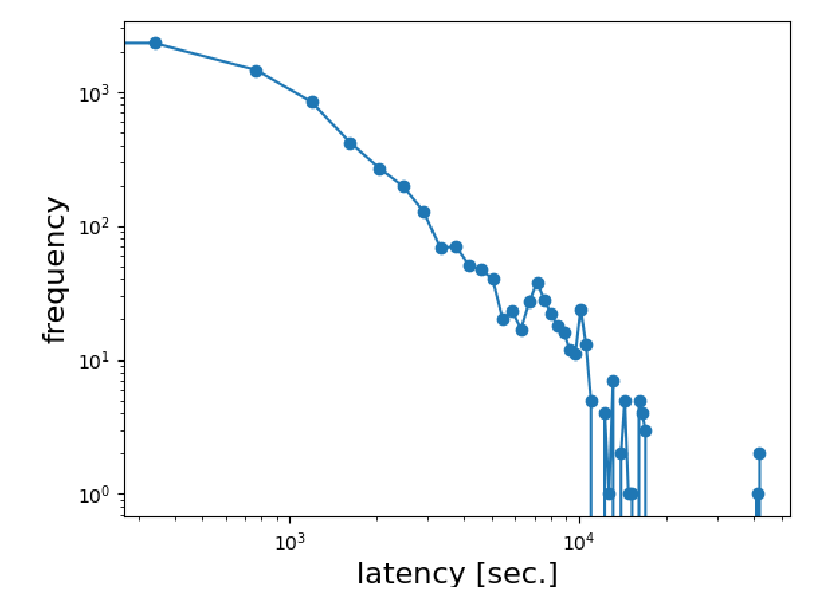
\includegraphics[width=85mm]{exp3-2.eps}
  \end{center}
  \vspace{20mm}
  \caption{取引送信からBCに取り込まれるまでにかかる時間のヒストグラム}
  \label{fig:exp3-2}
  %  \ecaption{english caption is here}
\end{figure}
%
ブロック生成時間分布が指数分布に従うことから,半日程度の短期間では
BCに取り込まれる時間は指数分布に従うが,1週間程度の長期間になると
指数分布から外れてくる.
実際に図\ref{fig:exp3-2}のとおり両対数プロットで直線的な傾向が現れる
為,冪分布に従う傾向が現れていることが確認できる.
また冪指数を両対数プロットの傾きから見積もると3/2に近いことが分かる.
これらの結果は優先権付き待ち行列の理論解析結果と矛盾しない.
このことから手数料の低い取引が優先度が低くなり,BCに取り込まれるまで
に時間がかかっていることが予想される.

取引サイズに対する取引手数料の割合と取引がBCに取り込まれるまでに
かかった時間の関係を図\ref{fig:exp3-3}に示す.
%
\begin{figure}[tb]
  \vspace{-20mm}
  \begin{center}
    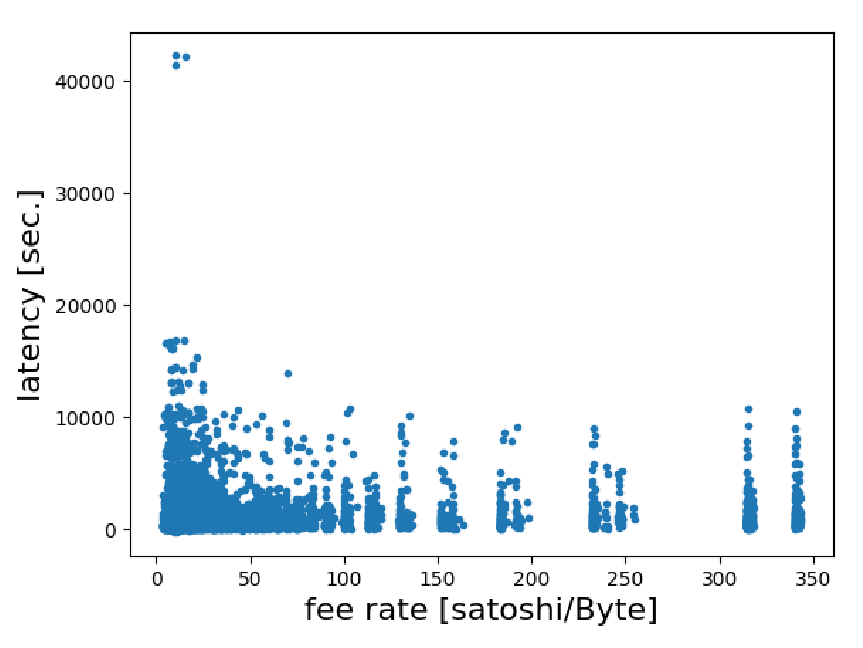
\includegraphics[width=85mm]{exp3-3.eps}
  \end{center}
  \vspace{20mm}
  \caption{取引サイズに対する取引手数料の割合と取引がBCに取り込まれるまでにかかった時間の関係}
  \label{fig:exp3-3}
  %  \ecaption{english caption is here}
\end{figure}
%
割合(fee rate)が低いとBCに取引が取り込まれるまでに時間がかかって
いることが分かる.このことからSTNにおいても優先権付き待ち行列理論
による考察は有効であると考えられる.








\section{Discussion}
\label{sec:discussion}



\section{Conclusion}
\label{sec:conclusion}


本研究ではBitcoin STNのノードを構築し,ブロックサイズの上限を撤廃
した環境における取引処理に関するデータ分析や性能評価実験を行った.
取引処理の稼働率の時間変化を調べた結果,推定稼働率は殆どの時間帯
において1を超えていることが分かった.
bitcoin-cliの機能を用いてBCの分岐確率の推定も行った結果,
STNでは約8.5\%となり,BTCの4倍超の確率となっていることが分かった.
またP2Pネットワークの平均ブロック転送時間も約53秒と推定できた.
OP\_RETURNスクリプトを含む取引を1分に1回の高頻度で1週間の期間,
転送することで取引処理性能を実験的に評価した.
その結果,取引がBCに取り込まれる確率は98\%であり,その時間分布は
長期的には冪分布に従うような傾向が確認できた.また優先権付き待ち
行列の理論と矛盾しない3/2の冪指数に従う傾向も確認できた.
このことからSTNにおいても優先権付き待ち行列理論による考察は有効
であると言える.

今後の課題としては,より大量な数の取引を長期間に渡って送信し続け
た時の処理性能について確認することが挙げられる.




\begin{acknowledgement}
 This work was partially supported by the Japan Society for the Promotion of 
Science (JSPS) through KAKENHI (Grants-in-Aid for Scientific Research) Grant 
Numbers 17H01742 and 20K11797. 
\end{acknowledgement}



%%
%\section*{Appendix}
%\addcontentsline{toc}{section}{Appendix}
%%
%%
%When placed at the end of a chapter or contribution (as opposed to at the end of the book), the numbering of tables, figures, and equations in the appendix section continues on from that in the main text. Hence please \textit{do not} use the \verb|appendix| command when writing an appendix at the end of your chapter or contribution. If there is only one the appendix is designated ``Appendix'', or ``Appendix 1'', or ``Appendix 2'', etc. if there is more than one.
%
%\begin{equation}
%a \times b = c
%\end{equation}


\begin{thebibliography}{99}

% Bitcoin
\bibitem{nakamoto}
  S. Nakamoto, 
  ``Bitcoin: A Peer-to-Peer Electronic Cash System''
  (White paper), 2008 
  \url{https://bitcoin.org/bitcoin.pdf} \ 
  \url{https://craigwright.net/bitcoin-white-}\\
  \url{paper.pdf}
  (2021年2月9日閲覧確認)


\bibitem{btc}
  Bitcoin Core 
  \url{https://github.com/bitcoin/bitcoin}
  (2021年2月9日閲覧確認)


\bibitem{ZHZB2020}
  Q. Zhou, \textit{et al.}, 
  ``Solutions to Scalability of Blockchain: A Survey''
  IEEE Access, Vol. 8, pp.16440-16455, IEEE, 2020. 


\bibitem{PD2016}
  J. Poon and T. Dryja, 
  ``The Bitcoin Lightning Network: Scalable Off-Chain Instant Payments,'' 
  (2016) \url{https://lightning.network/lightning-network-paper.pdf}
  (2021年2月9日閲覧確認)


\bibitem{silkroad}
  FBI, 
  ``Manhattan U.S. Attorney Announces Seizure of Additional \$28 Million 
    Worth of Bitcoins Belonging to Ross William Ulbricht, Alleged Owner 
    and Operator of ``Silk Road'' Website, '' 2013.
  \url{https://archives.fbi.gov/archives/newyork/press-releases/2013/manhattan-u.s.}\\
  \url{-attorney-announces-seizure-of-additional-28-millio}\\
  \url{n-worth-of-bitcoins-belonging-to-ross-william-ulbri}\\
  \url{cht-alleged-owner-and-operator-of-silk-road-website}
  (2021年2月9日閲覧確認)

\bibitem{alphabay}
  The US Department of Justice,
  ``AlphaBay, the Largest Online 'Dark Market,' Shut Down,'' 2017.
  \url{https://www.justice.gov/opa/pr/alphabay-largest-online-dark-mar}\\
  \url{ket-shut-down}
  (2021年2月9日閲覧確認)

\bibitem{welcome2video}
  The US Department of Justice,
  ``South Korean National and Hundreds of Others Charged Worldwide in the Takedown 
    of the Largest Darknet Child Pornography Website, Which was Funded by Bitcoin,'' 
  2019.
  \url{https://www.justice.gov/opa/pr/south-korean-national-and-hundreds-others-ch}\\
  \url{arged-worldwide-takedown-largest-darknet-child}
  (2021年2月9日閲覧確認)


% Blockchain for AI
\bibitem{SMNA2019}
  K. Salah, M. Habib Ur Rehman, N. Nizamuddin, and A. Al-Fuqaha,
  ``Blockchain for AI: Review and Open Research Challenges''
  IEEE Access, Vol. 7, pp.10127-10149, 2019.


\bibitem{bloX}
  U. Klarman, \textit{et al.},
  ``bloXroute: A Scalable Trustless Blockchain Distribution Network''
  (White paper), 2018.
  \url{https://bloxroute.com/wp-content/uploads/2018/03/blo}\\
  \url{Xroute-whitepaper.pdf}
  (2021年2月9日閲覧確認)


\bibitem{bsv}
  Bitcoin SV (Satoshi Vision) 
  \url{https://github.com/bitcoin-}\\
  \url{sv/bitcoin-sv}
  (2021年2月9日閲覧確認)

\bibitem{bitcoinscaling}
  Bitcoin Scaling Test Network
  \url{https://bitcoinscaling.io/}
  (2021年2月9日閲覧確認)


%\bibitem{fujihara2019}
%  A. Fujihara,
%  ``PoWaP: Proof of Work at Proximity for a crowdsensing system for 
%  collaborative traffic information gathering,'' 
%  Internet of Things, 100046, Elsevier (2019).
%  \url{https://www.sciencedirect.com/science/article/pii/S254266051830177X}
%
%\bibitem{Fujihara2018}
%  A. Fujihara,
%  ``Proposing a System for Collaborative Traffic Information Gathering and 
%  Sharing Incentivized by Blockchain Technology,''
%  The 10th International Conference on Intelligent Networking and 
%  Collaborative Systems (INCoS-2018), pp.170-182 (2018)
%  \url{https://link.springer.com/chapter/10.1007/978-3-319-98557-2_16}
%
%\bibitem{YF2020}
%  T. Yanagihara and A. Fujihara,
%  ``Experimental performance evaluation of cross-referencing method for 
%    multiple blockchains,'' 
%  IEICE Technical Report IN2019-129, pp.363-368 (2020)
%  \url{https://www.ieice.org/ken/paper/2020030611wm/eng/} (Japanese)


\bibitem{OB2005}
  J. G. Oliveira and A.-L. Barab\'asi,
  ``Darwin and Einstein correspondence patterns,'' 
  Nature 437, 1251, 2005.


\bibitem{KK2019}
  S. Kasahara and J. Kawahara,
  ``Effect of Bitcoin fee on transaction-confirmation process,''
  Journal of Industrial and Management Optimization, 15 (1): 365-386, 2019.


\bibitem{woc}
  WhatsOnChain.com, BSV Explorer - STN,
  \url{https://stn.whatsonchain.com/}
  (2021年2月9日閲覧確認)



% Flightradar24
\bibitem{flightradar24}
  Flight Tracker | Flightradar24 | Track Planes in Real-time,
  \url{https://www.flightradar24.com/}
  (2021年2月9日閲覧確認)





%% Block propagation delay
%\bibitem{DW2013}
%  C. Decker and R. Wattenhofer,
%  ``Information propagation in the Bitcoin network,''
%  IEEE P2P 2013 Proceedings, 2013.
%  \url{https://ieeexplore.ieee.org/abstract/document/6688704}
%
%% ghost 
%\bibitem{SZ2013}
%  Y. Sompolinsky and A. Zohar, 
%  ``Accelerating Bitcoin's Transaction Processing. Fast Money Grows on Trees, 
%  Not Chains'' (2013) 
%  \url{https://pdfs.semanticscholar.org/4016/80ef12c04c247c50737b9114c169c660aab9.pdf}
%
%
%
%\bibitem{SZ2015}
%  Y. Sompolinsky and A. Zohar, 
%  ``Secure High-Rate Transaction Processing in Bitcoin,''
%  FC 2015: Financial Cryptography and Data Security, International Conference 
%  on Financial Cryptography and Data Security, pp.507-527 (2015)
%  \url{https://eprint.iacr.org/2013/881.pdf}


\end{thebibliography}

\end{document}
